\documentclass{article}
\usepackage{spikey}
\usepackage{amsmath}
\usepackage{mathrsfs}
\usepackage{amssymb}
\usepackage{soul}
\usepackage{float}
\usepackage{graphicx}
\usepackage{hyperref}
\usepackage{fancyhdr}
\usepackage{xcolor}
\usepackage{chngcntr}
\usepackage{centernot}
\usepackage[shortlabels]{enumitem}
\usepackage[margin=1truein]{geometry}
\usepackage{tkz-graph}
\usepackage{dsfont}
\usepackage{caption}
\usepackage{subcaption}
\usepackage{booktabs}
\usepackage[yyyymmdd,hhmmss]{datetime}

\usepackage{tikz}
\usetikzlibrary{arrows}

\usepackage{setspace}
\linespread{1.15}
\usepackage[margin=1truein]{geometry}

\counterwithin{equation}{section}
\counterwithin{figure}{section}

\usepackage{listings}
 
\definecolor{codegreen}{rgb}{0,0.6,0}
\definecolor{codegray}{rgb}{0.5,0.5,0.5}
\definecolor{codeblue}{rgb}{0.3,0.5,0.8}
\definecolor{codepurple}{rgb}{0.58,0,0.82}
%\definecolor{backcolour}{rgb}{0.95,0.95,0.92}
\definecolor{backcolour}{rgb}{1,1,1}

\lstdefinestyle{mystyle}{
    backgroundcolor=\color{backcolour},   
    commentstyle=\color{codegreen},
    keywordstyle=\color{magenta},
    numberstyle=\tiny\color{codegray},
    stringstyle=\color{codepurple},
    basicstyle=\ttfamily\footnotesize,
    breakatwhitespace=false,         
    breaklines=true,                 
    captionpos=b,                    
    keepspaces=true,                 
    numbers=left,                    
    numbersep=5pt,                  
    showspaces=false,                
    showstringspaces=false,
    showtabs=false,                  
    tabsize=4
}

\lstset{style=mystyle}

\title{CSC413: Homework 3}
\date{\today\ at \currenttime}
\author{Tianyu Du (1003801647)}
\begin{document}
	\maketitle
	\section{Weight Decay}
	\subsection{Under-parameterized Model [0pt]}
	\begin{proof}[Solution]
		Given
	\begin{align}
		\mathcal{J}(\hat{\mathbf{w}})&=\frac{1}{2 n}\|X \hat{\mathbf{w}}-\mathbf{t}\|_{2}^2
		+\frac{\lambda}{2} \hat{\mathbf{w}}^{T} \hat{\mathbf{w}} \\
		\mathcal{J}(\hat{\mathbf{w}})&=\frac{1}{2 n}\|X \hat{\mathbf{w}}-\mathbf{t}\|_{2}^2
		+\frac{\lambda}{2} \norm{\hat{\vew}}_2^2
	\end{align}
	The gradient descent converges when $\frac{d}{d\hat{\vew}} \mathcal{J}(\hat{\mathbf{w}}) = 0$. Altogether with the fact that $\frac{d}{d\vex} \norm{\vex}_2^2 = 2 \vex^T$, the training converges if and only if:
	\begin{align}
		\frac{d}{d\hat{\vew}} \mathcal{J}(\hat{\mathbf{w}})
		&= \frac{1}{n} (X \hat{\vew} - \vet)^T X + \lambda \hat{\vew}^T \\
		&= \frac{1}{n} \hat{\vew}^T X^T X - \frac{1}{n} \vet^T X + \lambda \hat{\vew}^T = 0\quad (\dagger)
	\end{align}
	Note that when $d \leq n$, $rank(X) = d$ implies $X^T X$ is invertible. Suppose $X^T X + n \lambda I$ is invertible as well. Therefore,
	\begin{align}
		(\dagger) &\implies \left(\hat{\vew}^T X^T X + n \lambda \hat{\vew}^T \right) = \vet^T X \\
		&\implies \hat{\vew}^T \left(X^T X + n \lambda I \right) = \vet^T X \\
		&\implies \hat{\vew}^T = \vet^T X \left(X^T X + n \lambda I \right)^{-1} \\
		&\implies \hat{\vew} = \left(X^T X + n \lambda I \right)^{-1} X^T \vet
	\end{align}
	\end{proof}
	
	\subsection{Over-parameterized Model}
	\subsubsection{Warmup: Visualizing Weight Decay [1pt]}
	\begin{proof}[Solution]
		Given 
		\begin{align}
			\vex_1 = (2, 1)\tx{ and } t_1 = 2.
		\end{align}
		From previous homework, the solution of gradient descent without regularization is
		\begin{align}
			\vew^* = \left(\frac{4}{5}, \frac{2}{5} \right)
		\end{align}
		From the previous part, the gradient descent converges if and only if
		\begin{align}
			\frac{d}{d\hat{\vew}} \mathcal{J}(\hat{\mathbf{w}})
			&= \frac{1}{n} (X \hat{\vew} - \vet)^T X + \lambda \hat{\vew}^T \\
			&= ((2,1)\cdot (w_1, w_2) - 2) (2, 1) + \lambda (w_1, w_2) \\
			&= (2 w_1 + w_2 - 2) (2, 1) + (\lambda w_1, \lambda w_2) = 0 \\
		\end{align}
		Therefore, the solution to gradient descent with weight decay is:
		\begin{align}
			&\begin{cases}
				4 w_1 + 2 w_2 -4 + \lambda w_1 &= 0 \\
				2 w_1 + w_2 - 2 + \lambda w_2 &= 0
			\end{cases} \\
			\implies &\begin{cases}
				w_1^* &= \frac{4}{\lambda +5} \\
				w_2^* &= \frac{2}{\lambda +5}
			\end{cases}
		\end{align}
%		The solution space is parameterized by $\lambda$ as following
%		\begin{align}
%			\mc{S} := \left \{
%			\frac{4}{\lambda +5}, \frac{2}{\lambda +5}: \lambda \in \R_+
%			\right \}
%		\end{align}
%		which is a singleton uniquely determined by $\lambda$. Note that the following visualization assumes $\lambda = 1$.
		\begin{figure}[H]
			\centering
			\small
			\caption{Visualization}
			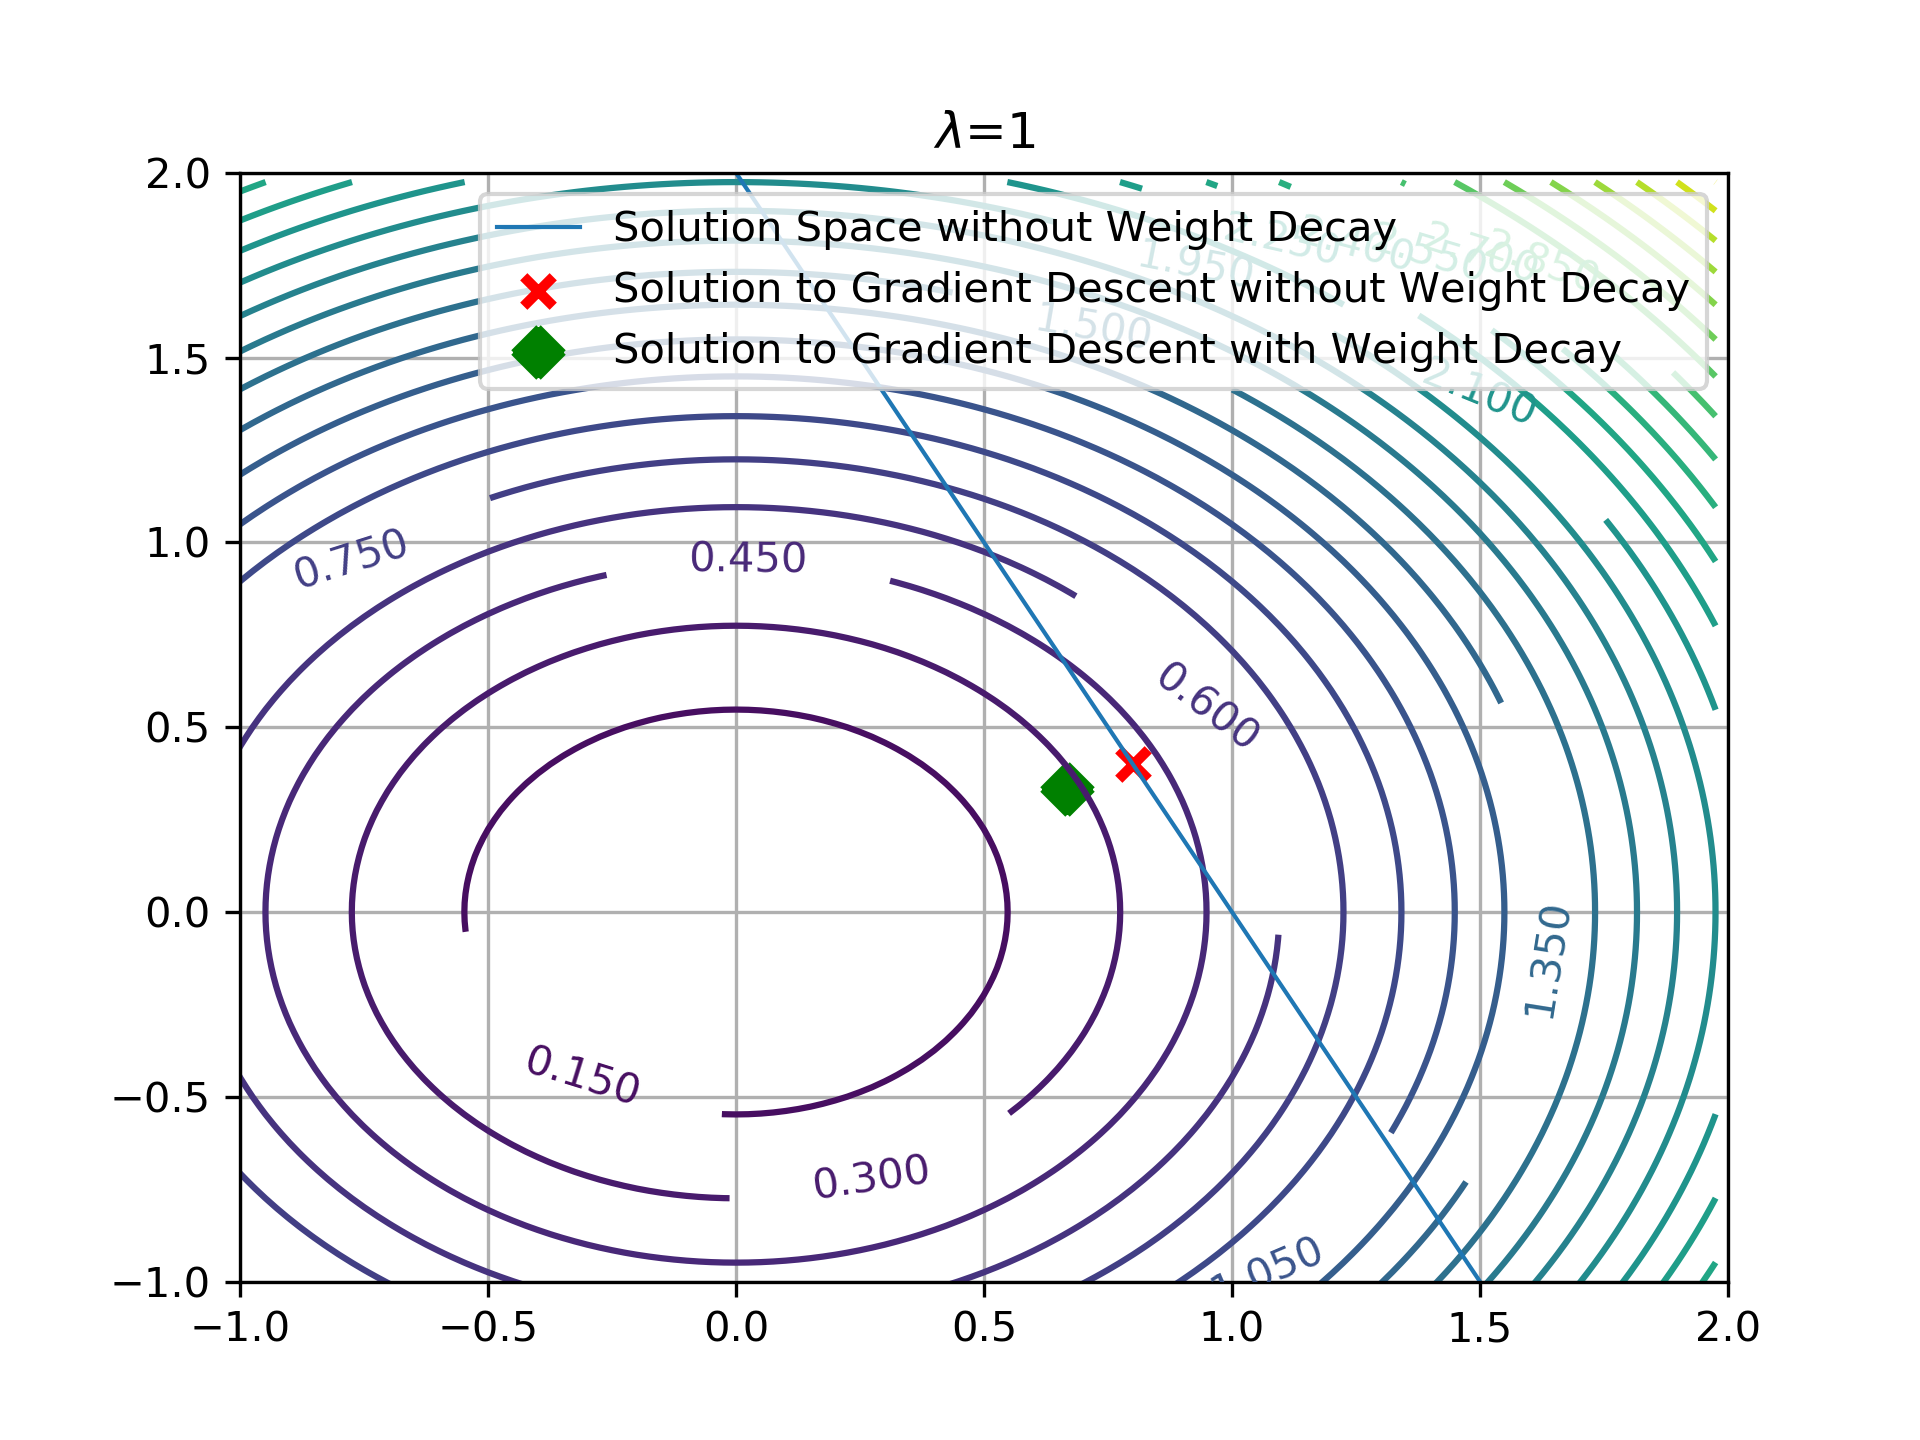
\includegraphics[width=\linewidth]{plot_q1.png}
		\end{figure}
	\end{proof}
	
	\subsubsection{Gradient Descent and Weight Decay [0pt]}
	\begin{proof}[Solution]
		The solution to gradient descent with weight decay at rate $\lambda$ has been derived in the previous section:
		\begin{align}
			\vew^{*\lambda}_\tx{weight decay} = \left(\frac{4}{\lambda +5}, \frac{2}{\lambda +5}\right)
		\end{align}
	\end{proof}
	
	\subsection{Adaptive optimizer and Weight Decay [1pt]}
	\begin{proof}[Solution]
		Note that the original loss function,
		\begin{align}
			\mathcal{J}(\hat{\mathbf{w}})=\frac{1}{2 n}\|X \hat{\mathbf{w}}-\mathbf{t}\|_{2}^{2}
		\end{align}
		is a convex function since its a composite of convex function $\norm{\cdot}_2^2$ and linear function $X \hat{\vew} - \textbf{t}$. Further, note that for any $\theta \in (0, 1)$ and $\vex \neq \vey$:
		\begin{align}
			&\theta \norm{\vex}_2^2 + (1 - \theta) \norm{\vey}_2^2 - \norm{\theta \vex + (1 - \theta) \vey}_2^2 \\
			&= \theta \norm{\vex}_2^2 + (1 - \theta) \norm{\vey}_2^2
			- \theta^2 \norm{\vex}_2^2 - (1 - \theta)^2 \norm{\vey}_2^2 - 2 \theta(1 - \theta) \inner{\vex}{\vey} \\
			&= \theta(1 - \theta) \norm{\vex}_2^2 + \theta (1 - \theta) \norm{\vey}_2^2
			- 2 \theta(1 - \theta) \inner{\vex}{\vey} \\
			&= \theta (1 - \theta) (\norm{\vex}_2^2 - 2\inner{\vex}{\vey} + \norm{\vey}_2^2) \\
			&= \theta (1 - \theta) \norm{\vex - \vey}_2^2 > 0
		\end{align}
		Therefore, $\norm{\vew}_2^2$ is strictly convex. The regularized loss function is a sum of convex and strictly convex functions, so it is strictly convex as well:
		\begin{align}
			\mathcal{J}(\hat{\mathbf{w}})=\frac{1}{2 n}\|X \hat{\mathbf{w}}-\mathbf{t}\|_{2}^{2}+\frac{\lambda}{2} \hat{\mathbf{w}}^{\top} \hat{\mathbf{w}}
		\end{align}
		Note that a strictly convex objective function has an (unique) global minimal, say $\vew^*$. Hence, conventional gradient descent methods, say SGD, will converge to $\vew^*$. Consider a SGD starting from $\vew_0 = \textbf{0}$, obviously
		\begin{align}
			\vew_0 \in Row(X)
		\end{align}
		and based on what we've shown in the previous homework,
		\begin{align}
			(X^T \vew - \textbf{t})^T X \in Row(X)
		\end{align}
		Therefore,
		\begin{align}
			\vew_1 = \vew_0 - \alpha (X^T \vew_0 - \textbf{t})^T X \in Row(X)
		\end{align}
		By induction, 
		\begin{align}
			\vew_{t+1} = \vew_t - \alpha (X^T \vew_t - \textbf{t})^T X \in Row(X)
		\end{align}
		Therefore, the weight SGD converges to $\vew^* \in Row(X)$. Since the objective function is strictly, so the minimizer is unique. Assuming Adagrad converges to the optimal solution, then Adagrad must converge to $\vew^*$, which is in $Row(X)$. Hence, Adagrad with regularization converges to $Row(X)$.
	\end{proof}
	
	
	\section{Ensembles and Bias-variance Decomposition}
	\subsection{Weight Average or Prediction Average?}
	\subsubsection{[1pt]}
	\begin{proof}[Solution]
		Suppose there are $K$ different models indexed using $j \in \{1, 2, \cdots, K\}$:
		\begin{align}
			h_j(\vex) = \vew_j(\mc{D}_j)\vex + b_j(\mc{D}_j)
		\end{align}
		where $\mc{D}_j$ are i.i.d. realization of datasets. Let $\overline{h}(\vex)$ denote the weight average ensemble:
		\begin{align}
			\overline{h}(\vex) &= \overline{\vew} \vex + \overline{b} \\
			&= \frac{1}{K} \left(\sum_{j=1}^K \vew_j(\mc{D}_j) \right) \vex + \frac{1}{K} \sum_{j=1}^K b_j(\mc{D}_j) \\
			&= \frac{1}{K} \left(\sum_{j=1}^K \vew_j(\mc{D}_j) \vex \right) + \frac{1}{K} \sum_{j=1}^K b_j(\mc{D}_j) \\
			&= \frac{1}{K} \left(
			\vew_j(\mc{D}_j) \vex + b_j(\mc{D}_j)
			\right) \\
			&= \frac{1}{K} \sum_{j=1}^K h_j(\vex)
		\end{align}
		which is the same as the prediction average at query point \vex.
		Therefore, the prediction from weight-average and prediction-average ensembles are the same. Hence, the expected generalization error should be the same.
	\end{proof}
	
	\subsubsection{[0pt]}
	\begin{proof}[Solution]
		
	\end{proof}
	
	\subsection{Bagging - Uncorrelated Models}
	\subsubsection{Bias with bagging [0pt]}
	\begin{proof}[Solution]
		Note that
		\begin{align}
			\expect{
				\bar{h}(\vex ; \mathcal{D})|\vex}
			&= \expect{
			\frac{1}{k} \sum_{i=1}^{k}
			h\left(\vex ; \mathcal{D}_{i}\right)
			| \vex} \\
			&= \frac{1}{k}
			\sum_{i=1}^{k}
			\expect{
			h\left(\vex ; \mathcal{D}_{i}\right)
			| \vex}
		\end{align}
		Since $\mc{D}_i$ are drawn from the identical distribution, so that
		\begin{align}
			\expect{
			h\left(\vex ; \mathcal{D}_{i}\right)
			| \vex} = 
			\expect{
			h\left(\vex ; \mathcal{D}_{j}\right)
			| \vex}\quad \forall i, j \in \{1, 2, \cdots, k\}
		\end{align}
		Hence,
		\begin{align}
			\expect{
				\bar{h}(\vex ; \mathcal{D})|\vex}
			= \frac{1}{k}
			\sum_{i=1}^{k}
			\expect{
			h\left(\vex ; \mathcal{D}_{i}\right)
			| \vex}
			= \expect{
			h\left(\vex ; \mathcal{D}_{i}\right)
			| \vex}\quad \forall i \in \{1, 2, \cdots, k\}
		\end{align}
		Since each data point in $\mc{D}_i$ is uniformly sampled with replaced from $\mc{D} \sim p_\tx{data}$, therefore, $\mc{D}_i \sim p_\tx{data}$ as well.
		\begin{align}
			\expect{
			h\left(\vex ; \mathcal{D}\right)
			| \vex}
			= 
			\expect{
			h\left(\vex ; \mathcal{D}_{i}\right)
			| \vex}\quad \forall i \in \{1, 2, \cdots, k\}
		\end{align}
		Therefore,
		\begin{align}
			bias = \expect{
			\abs{
			\expect{
				\bar{h}(\vex ; \mathcal{D})|\vex}
			- y_*(\vex)
			}^2
			}
			= \expect{
			\abs{
			\expect{
				h(\vex ; \mathcal{D})|\vex}
			- y_*(\vex)
			}^2
			}
		\end{align}
	\end{proof}
	
	\subsubsection{Variance with bagging [1pt]}
	\begin{proof}[Solution]
		Suppose 
		\begin{align}
			\expect{
				\abs{
					h(\vex; \mc{D})
					- \expect{h(x; \mc{D})|\vex}
				}^2
			} = \sigma^2
		\end{align}
		For the bagging model, 
		\begin{align}
			Var(\overline{h}) &= 
			\expect{
				\abs{
					\overline{h}(\vex; \mc{D})
					- \expect{\overline{h}(x; \mc{D})|\vex}
				}^2
			} \\
			&= 
			\expect{
				\abs{
				\frac{1}{k}
				\sum_{i=1}^{k}
				h\left(\vex ; \mathcal{D}_{i}\right)
					- \expect{\overline{h}(x; \mc{D})|\vex}
				}^2
			}\\
			&= \expect{
				\left(
				\frac{1}{k}
				\sum_{i=1}^{k}
				h\left(\vex ; \mathcal{D}_{i}\right)
					- \expect{\overline{h}(x; \mc{D})|\vex}
				\right)^2
			}
		\end{align}
		Since $\expect{\overline{h}(x; \mc{D})|\vex}$ is constant for all realizations of datasets $\mc{D}_i$ and equals $\expect{h(x; \mc{D})|\vex}$ by linearity of expectation.
		\begin{align}
			&= \expect{
				\left(
				\frac{1}{k}
				\sum_{i=1}^{k}
				\left\{h\left(\vex ; \mathcal{D}_{i}\right)
					- \expect{h(x; \mc{D}_i)|\vex}
				\right\}
				\right)^2
			} \\
			&= \frac{1}{k^2} \expect{
				\left(
				\sum_{i=1}^{k}
				\left\{h\left(\vex ; \mathcal{D}_{i}\right)
					- \expect{h(x; \mc{D}_i)|\vex}
				\right\}
				\right)^2
			}\quad (\dagger)
		\end{align}
		Because datasets $\mc{D}_i$ are drawn independently, 
		\begin{align}
			\expect{
				\left(h\left(\vex ; \mathcal{D}_{i}\right)
					- \expect{h(x; \mc{D}_i)|\vex}
				\right)
				\left(h\left(\vex ; \mathcal{D}_{j}\right)
					- \expect{h(x; \mc{D}_j)|\vex}
				\right)
			} = Cov(h_i, h_j) = 0
		\end{align}
		Hence, after expanding the squared sum in $(\dagger)$,
		\begin{align}
			(\dagger) &= \frac{1}{k^2} \expect{
				\sum_{i=1}^{k}
				\left(
				h\left(\vex ; \mathcal{D}_{i}\right)
					- \expect{h(x; \mc{D}_i)|\vex}
				\right)^2
			} \\
			&= \frac{1}{k^2} \sum_{i=1}^{k}
			\expect{
				\left(
				h\left(\vex ; \mathcal{D}_{i}\right)
					- \expect{h(x; \mc{D}_i)|\vex}
				\right)^2
			} \\
			&= \frac{1}{k^2} \sum_{i=1}^k Var(h_i)
		\end{align}
		Since $\mc{D}_i$ are i.i.d. from the dataset, $Var(h_i) = Var(h)$ for every $i$, therefore,
		\begin{align}
			Var(\overline{h}) &= \frac{\sigma^2}{k}
		\end{align}
	\end{proof}
	
	\subsection{Bagging - General Case}
	\subsubsection{Bias under Correlation [1pt]}
	\begin{proof}[Solution]
		The bias does not change and is independent from $\rho$. While deriving the bias, we firstly exchanged the expectation and summation using the linearity of summation operator:
		\begin{align}
			\expect{
				\bar{h}(\vex ; \mathcal{D})|\vex}
			&= \expect{
			\frac{1}{k} \sum_{i=1}^{k}
			h\left(\vex ; \mathcal{D}_{i}\right)
			| \vex} \\
			&= \frac{1}{k}
			\sum_{i=1}^{k}
			\expect{
			h\left(\vex ; \mathcal{D}_{i}\right)
			| \vex}
		\end{align}
		The linearity of expectation holds regardless of the correlation. Then we used the fact that $\mc{D}_i$ are identically distributed to show
		\begin{align}
			\frac{1}{k}
			\sum_{i=1}^{k}
			\expect{
			h\left(\vex ; \mathcal{D}_{i}\right)
			| \vex}
			= \expect{
			h\left(\vex ; \mathcal{D}\right)
			| \vex}
		\end{align}
		this step did not assume independent distribution. The entire proof (please refer to 2.2.1 for a more detailed derivation) did not use any assumption on distributional independence, hence the original proof is still valid in the general case.
	\end{proof}
	
	\subsubsection{Variance under Correlation [0pt]}
	\begin{proof}[Solution]
		\begin{align}
			Var(\bar{h}) &\equiv Cov\left(h(\vex;\mc{D}_i), h(\vex;\mc{D}_i)\right) \\
			&= Cov\left(\frac{1}{k} \sum_{i=1}^{k}
				h\left(\vex ; \mathcal{D}_{i}\right),
				\frac{1}{k} \sum_{i=1}^{k}
				h\left(\vex ; \mathcal{D}_{i}\right)\right) \\
			&= \frac{1}{k^2} Cov\left(\sum_{i=1}^{k}
				h\left(\vex ; \mathcal{D}_{i}\right),
				\sum_{i=1}^{k}
				h\left(\vex ; \mathcal{D}_{i}\right)\right) \\
			&= \frac{1}{k^2} \sum_{i=1}^{k} \sum_{j=1}^{k}
			Cov\left(
				h\left(\vex ; \mathcal{D}_{j}\right),
				h\left(\vex ; \mathcal{D}_{j}\right)\right) \\
			&= \frac{1}{k^2} \sum_{i=1}^{k} \sum_{j=1}^{k}
			Cov\left(
				h\left(\vex ; \mathcal{D}_{j}\right),
				h\left(\vex ; \mathcal{D}_{j}\right)\right) \\
			&= \frac{1}{k^2} (k \sigma^2 + (k^2-k) \rho \sigma^2) \\
			&= \left(
			\frac{1}{k} + \rho - \frac{\rho}{k}
			\right) \sigma^2 \\
			&= \left(
			\rho + \frac{1 - \rho}{k}
			\right) \sigma^2
		\end{align}
	\end{proof}
	
	\subsubsection{Intuitions on Bagging [1pt]}
	\begin{proof}{Solution}
		When $\rho = 1$, that is, all bootstrapped datasets are perfectly correlated. In fact, all datasets are identical, the variance is independent from $k$, and increasing number of estimators, $k$, does not help reduce the variance.
		
		However, For any $\rho < 1$, increasing number of estimators in the bagging, $k$, helps reduce the variance. In particular, when $\rho = 0$, which is the uncorrelated dataset case, the effect is most significant: the variance shrinks linearly in $k$. 
	\end{proof}
	
	\section{Generalization and Dropout}
	\subsection{Regression Coefficients}
	\subsubsection{Regression from $X_1$ [0pt]}
	\begin{proof}[Solution]
	\end{proof}
	
	\subsubsection{Regression from $X_2$ [1pt]}
	\begin{proof}[Solution]
		Since we are using $X_2$ only, equivalently, we can set the weight of $X_1$ to zero:
		\begin{align}
			\mc{J} &= \expe_{(x_2, y) \sim (X_2, Y)} [(y - \hat{y})^2] \\
			&= \expe_{(x_2, y) \sim (X_2, Y)} [(y - w_2 x_2)^2] \\
			&= \expe_{(x_2, y) \sim (X_2, Y)} [(y - w_2 (y + Gaussian(0, 1)))^2] \\
			&= \expe_{(x_2, y) \sim (X_2, Y)} [((1 - w_2)y - w_2 Gaussian(0, 1) )^2] \\
			&= \expe_{(x_2, y) \sim (X_2, Y)} [((1 - w_2)y)^2] + w_2^2 \expe_{(x_2, y) \sim (X_2, Y)}[Gaussian(0, 1)^2] \\
			&= (1 - w_2)^2 \expe_{y \sim Y} [y^2] + w_2^2
		\end{align}
		Taking the gradient and solve the first order condition:
		\begin{align}
			&\nabla_{w_2} (1 - w_2)^2 \expe_{y \sim Y} [y^2] + w_2^2 = 0 \\
			&\implies - 2(1 - w_2) \expe_{y \sim Y} [y^2] + 2 w_2 = 0 \\
			&\implies \expe_{y \sim Y} [y^2] - w_2 \expe_{y \sim Y} [y^2] - w_2 = 0 \\
			&\implies \expe_{y \sim Y} [y^2] + w_2 (1- \expe_{y \sim Y} [y^2]) = 0 \\
			&\implies w_2 = \frac{\expe_{y \sim Y} [y^2]}{\expe_{y \sim Y} [y^2] + 1}
		\end{align}
		The expectation of $y^2$ is
		\begin{align}
			\expe_{y \sim Y} [y^2] &= \expe_{x_1 \sim X_1} (x_1 + Gaussian(0, \sigma^2))^2 \\
			&= 2 \sigma^2 \\
			\implies w_2 &= \frac{2 \sigma^2}{2 \sigma^2 + 1}
		\end{align}
	\end{proof}
	
	\subsubsection{Regression from $(X_1, X_2)$ [1pt]}
	\begin{proof}[Solution]
		Let $G_1, G_2, G_3$ denote the three Gaussian distributions respectively, so that
		\begin{align}
			X_1 &\leftarrow G_1 \\
			Y &\leftarrow X_1 + G_2 \\
			X_2 &\leftarrow Y + G_3
		\end{align}
		So that,
		\begin{align}
			\mc{J} &= \expe_{(x_1, x_2, y) \sim (X_1, X_2, Y)} [(y - \hat{y})^2] \\
			&= \expe [G_1 + G_2 - w_1 G_1 - w_2 (G_1 + G_2 + G_3)]^2 \\
			&= \expe [(1 - w_1 - w_2)G_1 + (1 - w_2)G_2 - w_2 G_3 ]^2 \\
			&= (1-w_1-w_2)^2 \sigma^2 + (1 - w_2)^2 \sigma^2 + w_2^2
		\end{align}
		For $w_1$:
		\begin{align}
			&\pd{}{w_1} \mc{J} = - 2 (1 - w_1 - w_2) \sigma^2 = 0
		\end{align}
		For $w_2$:
		\begin{align}
			&\pd{}{w_2} \mc{J}
			= - 2 (1 - w_1 - w_2) \sigma^2 
			- 2 (1 - w_2) \sigma^2
			+ 2 w_2 = 0 
		\end{align}
		Solving two equations:
		\begin{align}
			w_1 &= \frac{1}{\sigma ^2+1} \\
			w_2 &= \frac{\sigma ^2}{\sigma ^2+1}
		\end{align}
		The solution does not generalize well if $\sigma$ changes since both $w_1$ and $w_2$ depend on and are sensitive to $\sigma$.
	\end{proof}
	
	\subsubsection{Different $\sigma$s [0pt]}
	\begin{proof}[Solution]
		The expected loss can be re-written using law of total expectation as
		\begin{align}
			\mc{L}^2 &= \frac{1}{2} \expe_{(x_1, x_2, y) \sim (X_1, X_2, Y)} [(y - \hat{y})^2|\sigma=\sigma_1]
			+ \frac{1}{2} \expe_{(x_1, x_2, y) \sim (X_1, X_2, Y)} [(y - \hat{y})^2|\sigma=\sigma_2]
		\end{align}
		Therefore,	
		\begin{align}
			\sigma_*^2 &= \frac{\sigma_1^2 + \sigma_2^2}{2} \\
			\tx{and }
			w_1 &= \frac{1}{\sigma_*^2+1} \\
			w_2 &= \frac{\sigma_*^2}{\sigma_*^2+1}
		\end{align}
	\end{proof}
	
	\subsection{Dropout as Data-Dependent $L2$ Regularization}
	\subsubsection{Expectation and variance of predictions [0pt]}
	\begin{proof}[Solution]
		Let
		\begin{align}
			\tilde{y} &= 2\left(m_{1} w_{1} x_{1}+m_{2} w_{2} x_{2}\right)
		\end{align}
		Then
		\begin{align}
			\expect{\tilde{y}} &= \expect{2\left(m_{1} w_{1} x_{1}+m_{2} w_{2} x_{2}\right)}
		\end{align}
	\end{proof}
	
	\subsection{Effect on Dropout [1pt]}
	\begin{proof}[Solution]
	Using bias-variance decomposition of the generalization error while assuming zero irreducible error:
		\begin{align}
			\expe[\tilde{\mc{L}}]
			&= \expe [(\tilde{y} - y)^2] \\
			&= \expect{(\expe_m[\tilde{y}] - y)^2}
			+ Var(\hat{y}) \\
			&= \expe \left[(
				\hat{y} - y
			)^2 \right]
			+ Var(2\left(m_{1} w_{1} x_{1}+m_{2} w_{2} x_{2}\right)) \\
			&= \expe \left[(
				\hat{y} - y
			)^2 \right]
			+ 4Var\left(m_{1} w_{1} x_{1}+m_{2} w_{2} x_{2}\right) \\
			&= \expe \left[(
				\hat{y} - y
			)^2 \right]
			+ 4Var\left(m_{1} w_{1} x_{1}\right)
			+ 4Var \left(m_{2} w_{2} x_{2}\right) \\
			&= \expe \left[(
				\hat{y} - y
			)^2 \right]
			+ Var(x_1) w_{1}^2
			+ Var(x_2) w_{2}^2 \\
			&= \expe \left[(
				\hat{y} - y
			)^2 \right]
			+ \sigma^2 w_{1}^2
			+ (2 \sigma^2 + 1) w_{2}^2 \\
			&= (1-w_1-w_2)^2 \sigma^2 + (1 - w_2)^2 \sigma^2 + w_2^2
			+ \sigma^2 w_{1}^2
			+ (2 \sigma^2 + 1) w_{2}^2
		\end{align}
		Solving the first order condition $\nabla_{\vew} \mc{L} = 0$ gives
		\begin{align}
			\begin{cases}
				w_1 &= \frac{2 + 2 \sigma^2}{4+7\sigma^2} \\
				w_2 &= \frac{3 \sigma^2}{4+7\sigma^2}
			\end{cases}
		\end{align}
		The squared-norm $\vew_\tx{dropped out}$ is
		\begin{align}
			\norm{\vew_\tx{dropped out}}_2^2 = \frac{13 \sigma ^4+8 \sigma ^2+4}{\left(7 \sigma ^2+4\right)^2}
		\end{align}
		For the original solution:
		\begin{align}
			\norm{\vew_\tx{regular}}_2^2 = \frac{\sigma ^4+1}{\left(\sigma ^2+1\right)^2}
		\end{align}
		The ratio of two norms is
		\begin{align}
			r = \frac{\norm{\vew_\tx{dropped out}}_2^2}{\norm{\vew_\tx{regular}}_2^2} = \frac{\left(\sigma ^2+1\right)^2 \left(13 \sigma ^4+8 \sigma ^2+4\right)}{\left(7 \sigma ^2+4\right)^2 \left(\sigma ^4+1\right)}
		\end{align}
		For $\sigma \geq 0$, $r(\sigma)$ attains its maximal value of 0.417 at $\sigma \approx 1.11$. Hence, adding the dropout always reduce the norm of solution $\vew^*$, but does not necessarily reduce every entry in $\vew^*$.
		Therefore, adding the dropout is equivalent to adding a regularization term in which the level of plenty ($\lambda_j$) for each $w_j$ depends on the variance of $x_j$. In this case, $w_1$ is more regularized. And such regularization would help the model achieve a better generalization error.
	\end{proof}
	
	\section{Hard-Coding Recurrent Neural Networks [1pt]}
	\begin{proof}[Solution]
		Let $\sigma = \frac{1}{1 + \exp(-100\times z)}$, so that the sigmoid function behaves like an hard threshold indicator function $\id{x \geq 0}$. In the following part of my answer, I am considering $\sigma$ as a threshold function.
		Let $\vex_t = (x_1^t, x_2^t)$ denotes the input feature at time $t$. Note that when weights are sufficient large in scale, $\sigma$ behaves like hard threshold function.
		Consider the following recurrent network:
		\begin{align}
			\hat{y}_t &= \sigma(\vew_{hy} \veh_t + b_y)\\
			\veh_t &= \sigma\left(
				\vew_{xh} \vex_t
				+ \vew_{hh} \veh_{t-1}
				+ \veb_h
			\right)
		\end{align}
		with the following parameters:
		\begin{align}
			\vew_{xh} &= 
			\begin{pmatrix}
				 1 & 1 \\
				 1 & 1 \\
				 1 & 1
			\end{pmatrix}
			\quad
			\vew_{hh} = 
			\begin{pmatrix}
				0 & 1 & 0 \\
				0 & 1 & 0 \\
				0 & 1 & 0
			\end{pmatrix}
			\quad
			\veb_h = \begin{pmatrix}
				-0.5 \\ -1.5 \\ -2.5
			\end{pmatrix}
		\end{align}
		\begin{align}
			\vew_{hy} = 
			\begin{pmatrix}
				1 & -1 & 1
			\end{pmatrix}
			\quad
			b_y = -0.5
		\end{align}
		
		\begin{align}
			\veh_t = 
			\begin{pmatrix}
				\id{x_1^t + x_2^t + h_{t-1} \geq 1} \\
				\id{x_1^t + x_2^t + h_{t-1} \geq 2} \\
				\id{x_1^t + x_2^t + h_{t-1} \geq 3}
			\end{pmatrix}
		\end{align}
		\emph{Justification:} \\
		\begin{align}
			\vew_{xh} \vex_t =
			\begin{pmatrix}
				x_1^t + x_2^t \\
				x_1^t + x_2^t \\
				x_1^t + x_2^t \\
			\end{pmatrix} \quad
			\vew_{hh} \veh_{t-1} =  
			\begin{pmatrix}
				\id{x_1^{t-1} + x_2^{t-1} + h_{t-2} \geq 2} \\
				\id{x_1^{t-1} + x_2^{t-1} + h_{t-2} \geq 2} \\
				\id{x_1^{t-1} + x_2^{t-1} + h_{t-2} \geq 2} \\
			\end{pmatrix}
		\end{align}
		Let $c_t$ denote the carry from the previous significant figure. Therefore, elements in $\vew_{hh} \veh_{t-1}$ are one only if $c_t = 1$.
		Then,
		\begin{align}
			\veh_t
			= \sigma\left(
				\vew_{xh} \vex_t
				+ \vew_{hh} \veh_{t-1}
				+ \veb_h
			\right)
			= \begin{pmatrix}
				\id{x_1^t + x_2^t + c_t \geq 1} \\
				\id{x_1^t + x_2^t + c_t \geq 2} \\
				\id{x_1^t + x_2^t + c_t \geq 3}
			\end{pmatrix}
		\end{align}
		For the output layer, 
		\begin{align}
			\hat{y}_t = \sigma\left(
				\vew_{xh} \vex_t
				+ \vew_{hh} \veh_{t-1}
				+ \veb_h
			\right) = \id{x_1^t + x_2^t + c_t \geq 1} \lor \id{x_1^t + x_2^t + c_t \geq 3}
		\end{align}
		Therefore, let $c \in \{0, 1\}$ denote the carry, $\hat{y}$ whenever $x_1 + x_2 + c$ is one or three, and $\hat{y} = 0$ otherwise.
	\end{proof}
\end{document}






























